% !TEX encoding = UTF-8 Unicode

\documentclass[a4paper]{article}

\usepackage{color}
\usepackage{url}
\usepackage[T2A]{fontenc} % enable Cyrillic fonts
\usepackage[utf8]{inputenc} % make weird characters work
\usepackage{graphicx}
\usepackage{placeins}
\graphicspath{ {./slike/} }
\documentclass{article}
\usepackage[utf8]{inputenc}
\usepackage[serbian]{babel}
\usepackage[margin=3.5cm, left=3cm, right=3cm, top=1cm, headheight=1cm, headsep=0.8cm, footskip=1.2cm, bottom=1.5cm, includefoot, includehead]{geometry} 
\usepackage{graphicx}
\usepackage{amsmath}
\newtheorem{exercise}{\Large Zadatak}
\usepackage[export]{adjustbox}
\usepackage{caption}
\usepackage{subcaption}
\usepackage{fancyhdr}
\usepackage[bottom]{footmisc}
\pagestyle{fancy}
\usepackage[figurename=Slika]{caption}
\usepackage[serbian]{babel}
\fancyhf{}
\usepackage{gensymb} 
\author{Andrijana Aleksić}
\usepackage{fancyhdr}
\pagestyle{fancy}
\makeatletter
\let\runauthor\@author
\let\runtitle\@title
\makeatother
\lhead{\runauthor}
\rhead{Primene dubokog učenja u lečenju 
karcinoma }
%\usepackage[english,serbianc]{babel} %ukljuciti babel sa ovim opcijama, umesto gornjim, ukoliko se koristi cirilica

\usepackage[unicode]{hyperref}
\hypersetup{colorlinks,citecolor=green,filecolor=green,linkcolor=blue,urlcolor=blue}

%\newtheorem{primer}{Пример}[section] %ćirilični primer
\newtheorem{primer}{Primer}[section]

\begin{document}

\title{Primene dubokog učenja u lečenju 
karcinoma\\ 

\bigskip
\small{Seminarski rad
\\Računarstvo i društvo
\\ Matematički fakultet}}

\author{Andrijana Aleksić}
\date{jul, 2022.}
\maketitle



\newpage

\tableofcontents

\newpage

\section{Uvod}
\label{sec:uvod}
Nova tehnologija dubokog učenja koja je najzastupljenija u računarskim naukama (computer science), sada ima i razvija primene u mnogim drugim granama kao što su robotika, snimanje karcinoma, procesiranje jezika (prirodnih), računarski vid.\cite{goodfellow}.
U domenu mašinskog učenja, duboko učenje je porodica računarskih metoda koja omogućava algoritmu da programira sebe učeći na velikom skupu primera koji demonstriraju željeno ponašanje, uklanjajući potrebu za eksplicitnim definisanjem pravila \cite{lafrate}.

Cilj ovog rada je da se analiziraju studije tehnologija dubokog učenja u snimanju karcinoma i studija koje mogu da podstaknu promenu primenjivanih tehnologija u kliničkoj onkologiji i poboljšaju dijagnostiku i lečenje karcinoma.

Rad će se fokusirati na studije slučaja primene tahnologija dubokog učenja na detekciju karcinoma pluća i grudi koji su dve najuticajnije bolesti u društvu. 

Takođe, rad će analizirati stanje novih tehnologija za tri vrste karcinoma (pluća, grudi, štitna žlezda) i izvore ovih novih tehnologija na nivou polja istraživanja na kojim nastaju, univerziteta i država koje imaju najveću naučnu proizvodnju. 

Diskusija na kraju rada prikazaće socio-ekonomske barijere za primenu novih tehnologija dubokog učenja u medicini.

Vrednost ovih istraživanja je u tome što prikazuje da nove tehnologije mogu doprineti poboljšanju lečenju karcinoma, ali zahteva dodatnu velidaciju, ponovljivost i mogućnost uopštenja primenjivih tehnika.

\section{Studije slučaja}
\label{sec:naslov1} 

Prikazane su dve studije slučaja algoritama dubokog učenja u snimanju karcinoma. Date studije su:

\begin{itemize}
    \item Tehnologija dubokog učenja za detekciju različitih vrsta karcinoma pluća
    \item Tehnologija dubokog učenja za procenu metastaze limfnih čvorova kod karcinoma dojke
\end{itemize}

\subsection{Duboko učenje za detekciju tipa karcinoma pluća}
\label{subsec:podnaslov1}


Karcinom pluća je jedna od glavnih bolesti u ogromnom broju država i glavni uzrok smrti u odnosu na oba pola. Karcinom pluća izazivaju pušenje, pasivno pušenje, zagađenje vazduha, itd. Mortalitet ovog karcinoma je visok i stopa preživljanja pacijenta u roku od 5 godina iznosi 2-10\% \cite{bray}. Detekcija tipa karcinoma i mutacije je kritični dijagnostički proces za omogućivanje adekvatnog lečenja \cite{coccia}.

Trenutni pristup precizne dijagnoze zasniva se na molekularnim biomarkerima na plućnoj biopsiji i testovima krvi. Ovaj pristup može da precizno dijagnostifikuje tip i mutaciju karcinoma pluća, ali ima i negativnih strana. Metode zahtevaju invazivne hiruške zahvate, vreme čekanja do početka lečenja može premašiti mesec dana, takođe, bolnicama predstavlja veliki trošak zbog potreba biopsije i odgovarajuće opreme.

U \cite{coudray} je razvijen model dubokog učenja za automatsku analizu snimaka tumora koristeći javno dostupne snimke iz \emph{Atlasa genoma kancera}. Model vrši trostruku klasifikaciju u klase normalnog tkiva, plućnog adenokarcinoma i rožnatog plućnog karcinoma. Njegovi rezultati su upoređeni sa rezultatima troje patologa koji klasifikovali isti skup podataka na osnovu vizualne inspekcije. Performanse modela su bile uporedive sa performansama patologa, što je dokazalo da ove tehnologije mogu da asistiraju patolozima u detekciji podtipova karcinoma. Primenom ove metode može se smanjiti cena dijagnoze i omogućiti siromašnijim regionima da dođu do dobrih dijagnoza slanjem snimaka tumora.

\newpage
\subsection{Duboko učenje za detekciju metastaze kod karcinoma dojke}
\label{subsec:podnaslov2}

Karcinom dojke je najčešći oblik među ženama. Studije rađene u naprednijim zemljama pokazuju da je sve veći broj obolelih od ove bolesti. Ovo može biti prouzrokovano ishranom, većim korišćenjem hormonskih terapija, oralnih kontraceptiva, kasnijim trudnoćama. \cite{coccia2}.

Metod biopsije dojki se koristi za dijagnozu svih tipova, stadijuma i mutacija karcinoma dojki, kao i kod drugih karcinoma.Osetljivost evaluacije limfnih čvorova od strane patologa nije optimalni proces odlučivanja. Neka istraživanja pokazuju da patološko razmatranje pogreši status limfnih čvorova kod 24\% pacijenata. Ovo se dešava zbog težine ljudskog odlučivanja u kompleksnim okolnostima. Dodatno, cena pregleda može biti skupa.

U \cite{ehteshami} otkriva se algoritam dubokog učenja koji je pokazao bolje performanse nego panel od 11 patologa koji su učestvovali u simulacionoj vežbi koja je dizajnirana da replicira rutinu patološkog rada. Dakle, eksperiment pokazuje da bi algoritam dubokog učenja mogao da identifikuje metastaze u limfnim čvorovima sa osetlljivošću od 100\%, dok je 40\% snimaka bez metastaza identifikovano korektno. Ovi rezultati bi mogli da se koriste u praksi kao deo organizacije kliničke prakse kako bi se smanjilo opterećenje patologa i poboljšalo njihovo odlučivanje vezano za adekvatnu terapiju.


\newpage
\section{Metode i Rezultati}
\label{sec:analiza}



\subsection{Metode}
\label{subsec:podnaslov3}

Ova studija, kao sto je pomenuto se bazirala na proucavanju primene algoritama dubokog ucenja za dva tipa karcinoma.
Korišćeni su podaci sa sajta ScienceDirect (2019). Na tom sajtu su upotrebljeni napredni algoritmi koji su izdvajali podatke pretraživanjem ključnih reči:

\begin{itemize}
    \item ``Deep learning" i ``lung cancer"
    \item ``Deep learning" i ``breast cancer"
    \item ``Deep learning" i ``thyroid cancer"
\end{itemize}

Odnos između broja istraživannja i godina je analiziran pomoću OLS (ordinary least squares) metode za procenu nepoznatih parametara u modelu linearne regresije.

Kao rezulatate, model daje: regresione keoficijente, prilagođen \begin{math}R^2\end{math}, standardnu grešku i procenjenu varijacionu tabelu.

Radi dalje procene rasta broja istraživanja iskorišćena je sledeća eksponencijalna forumula:

\begin{math}r = \frac{\log(\frac{P_{t(2018)}}{P_{0(1996)}})}{t}\end{math}, gde je

P = broj naučnih radova sa odgovarajućim kombinacijama termina

t = vreme (1996 do 2018)

r = brzina eksponencijalnog rasta broja radova

\bigskip

Dodatno, analizirani su izvori novih tehnologija u odnosu na njihovu naučnu oblast, univerzitete i države iz kojih potiču.


\subsection{Rezultati}
\label{subsec:podnaslov4}

\FloatBarrier
\subsubsection{Izvori tehnologija za karcinome pluća}
\label{subsec:ppnaslov2}



\begin{figure}[hbt!]
\centering
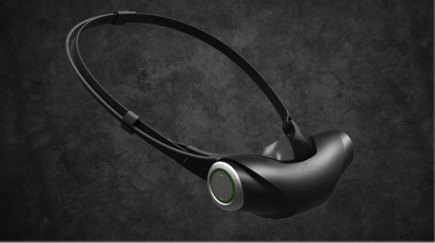
\includegraphics[width=8cm]{5.png}
\caption{Naučne oblasti radova primene dubokog učenja za karcinom pluća}
\end{figure}


\begin{figure}[hbt!]
\centering
\includegraphics[width=8cm]{6.png}
\caption{Produkcija naučnih studija tehnologija dubokog učenja za karcinom raka po državama}
\end{figure}


Na slici 1 su prikazane glavne oblasti istraživanja koje proizvode studije dubokog učenja za karcinom pluća, neke od oblasti su medicina, računarske nauke i inženjering.

Većina izvora na ovom polju dolazi u obliku članaka i konferencijskih radova, dok su vodeći univerziteti: Radbound Univerzitet Nijmegen Medicinski centar, Northwester Politehnički Univerzitet, Norheaster Univerzitet, Harvardski Medicinski fakultet, Ženska bolnica Kineske akademije nauka i Šangajski Jao Tong Univerzitet.

Vodeće države, sa najvećom produkcijom u ovom polju su SAD, Kina, Indija i Holandija (Slika 2).

Istraživanja na ovom polju tehnologija dubokog učenja su proizvela oko 6000 patenata do 2019. godine.


\FloatBarrier
\subsubsection{Izvori tehnologija za karcinome dojke}
\label{subsec:ppnaslov3}


\begin{figure}[hbt!]
\centering
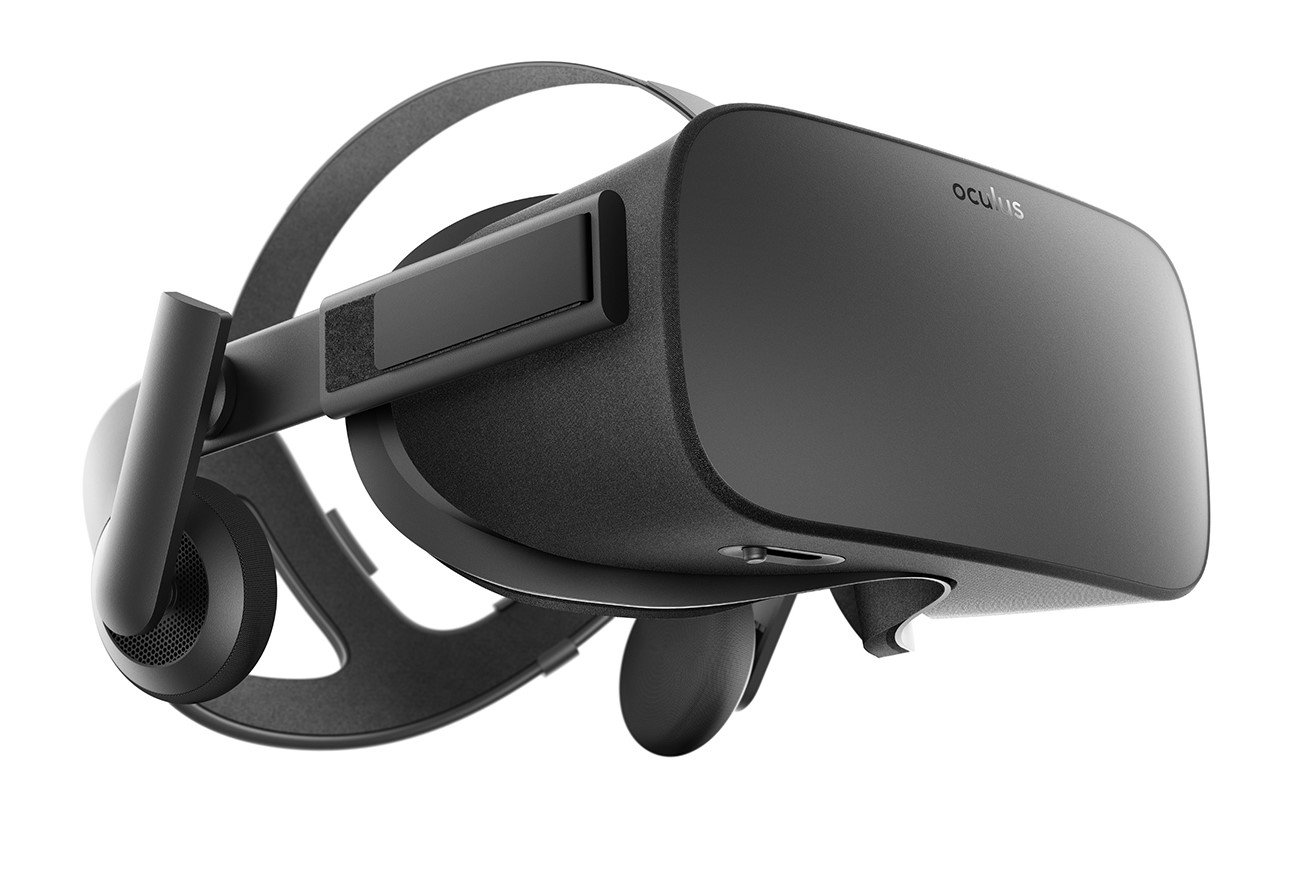
\includegraphics[width=8cm]{7.png}
\caption{Naučne oblasti radova primene dubokog učenja za karcinom dojke}
\end{figure}

\begin{figure}[hbt!]
\centering
\includegraphics[width=8cm]{8.png}
\caption{Produkcija naučnih studija tehnologija dubokog učenja za karcinom dojke po državama}
\end{figure}


Slika 3 prikazuje studije dubokog učenja u oblasti karcinoma grudi, tu se nameću studije iz oblasti medicine, informatike i inženjeringa.
Najveći broj informacija se dobija iz konferencijskih članaka i naučnih radova.

Univerziteti koji vode po broju istraživanja u ovoj oblasti su: Radboud Univerzitet, Nijmegen Medicinski Centar, Univerzitet Chicago, Univerzitet Pittsburgh,
Univerzitet Michigan (Ann Arbor), Case Western Reserve Univerzitet, Chinese Academy of Sciences,
Harvard Medical School i Univerzitet Michigan Medical School.

Slika 4 prikazuje da se najveći broj ovih istraživanja desava u SAD-u, Kini, Indiji i UK.


\FloatBarrier
\subsubsection{Izvori tehnologija za karcinome štitne žlezde}
\label{subsec:ppnaslov4}

\begin{figure}[hbt!]
\centering
\includegraphics[width=8cm]{9.png}
\caption{Naučne oblasti radova primene dubokog učenja za karcinom štitne žlezde}
\end{figure}

\begin{figure}[hbt!]
\centering
\includegraphics[width=8cm]{10.png}
\caption{Produkcija naučnih studija tehnologija dubokog učenja za karcinom štitne žlezde po državama}
\end{figure}

Vodeći univerziteti koji se bave proučavanjem karcinoma tiroidne zlezde su: Emory University School of Medicine, Georgia Institute, Medical College of Georgia, Rochester Institut i Univerzitet do Porto.

U slučaju ovog istraživanja vodece zemlje su SAD, Kina i Južna Koreja.


\FloatBarrier

\subsubsection{Analiza pravca tehnologija dubokog učenja}
\label{subsec:ppnaslov1}

\begin{figure}[hbt!]
\centering
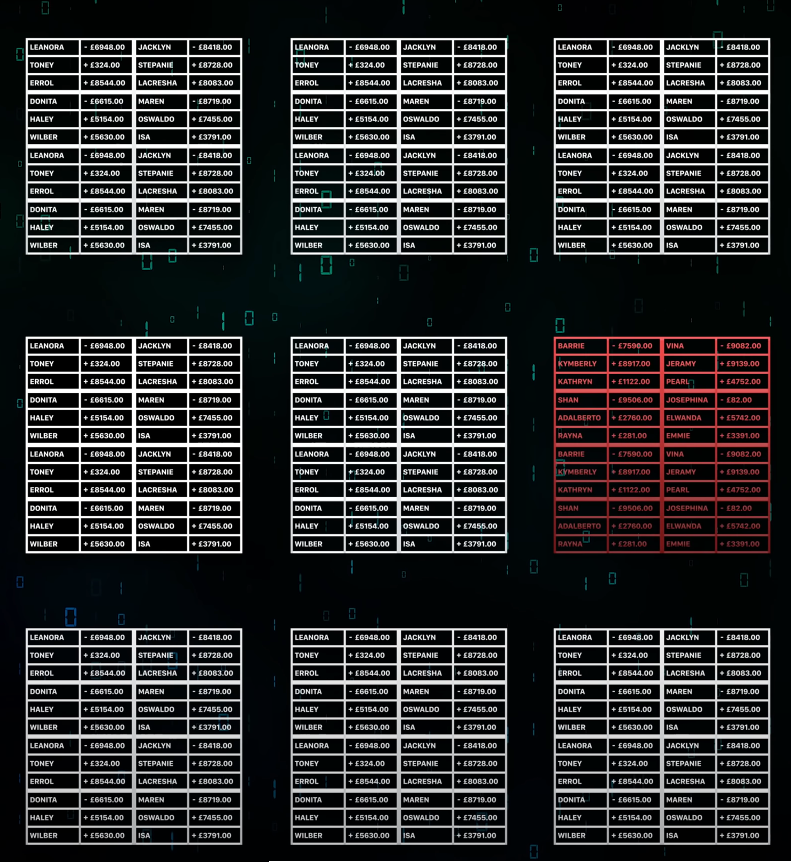
\includegraphics[width=8cm]{slika1.png}
\caption{Godišnji broj članaka o studijama dubokog učenja za različite vrste karcinoma (pluća, dojke, štitne žlezde)}
\end{figure}

\begin{figure}[hbt!]
\centering
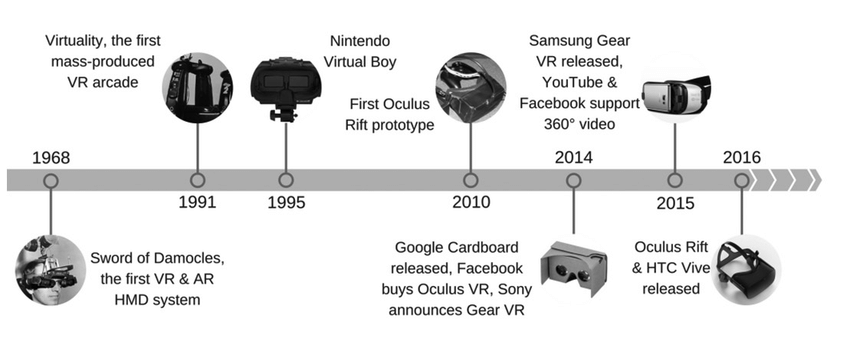
\includegraphics[width=8cm]{2.png}
\caption{Povratne vrednosti eksponencijalnog modela za različite vrste karcinoma}
\end{figure}



\begin{figure}[hbt!]
\centering
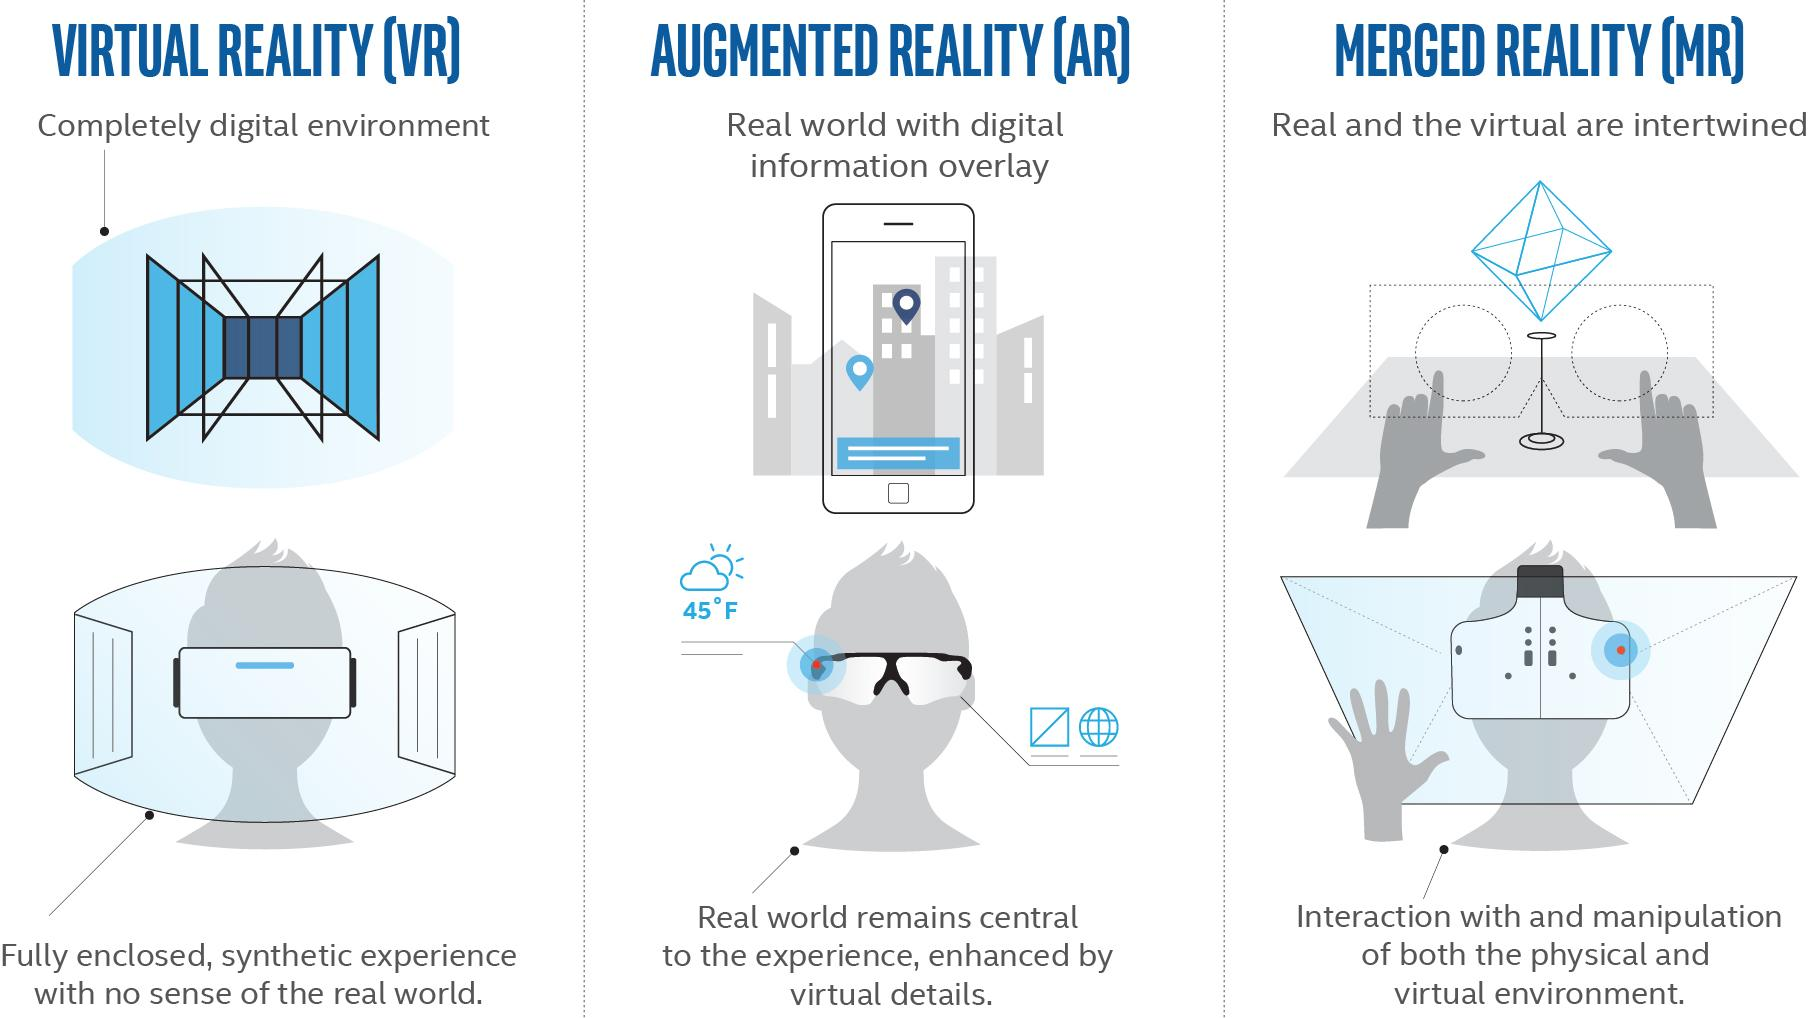
\includegraphics[width=8cm]{3.png}
\caption{Eksponencijalne krive broja članaka o studijama dubokog učenja za različite vrste karcinoma}
\end{figure}

\begin{figure}[hbt!]
\centering
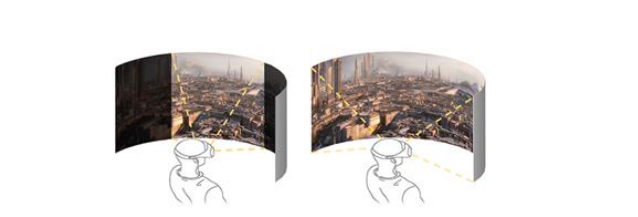
\includegraphics[width=8cm]{4.png}
\caption{Brzine eksponencijalnog rasta broja studija za rasličite vrste karcinoma}
\end{figure}

\newline
Ova četiri dijagrama (7-10) pokazuju da razvijanje tehnologija dubokog učenja u proučanju raka ima eksponencijalni rast koji je počeo 90-ih godina i dalje traje sa najvećim ubrzanjem kod karcinoma pluća i dojki. Dublja istraživanja govore da su nagli porasti broja istraživanja studija karcinoma pluća i dojki uslovljena većom stopom smrtnosti \cite{coccia2}. Sada se podstiče nastanak novih smerova u studijama karcinoma, kreirajuću osnovu za promenu prakse snimanja karcinoma koja bi mogla da vodi boljim dijagnozama i boljem lečenju.

\newpage
\section{Zaključak}
\label{sec:diskusija}

Tehnologije dubokog učenja mogu da daju podršku kliničkom procesu interpretacija snimaka, omogućavajući patolozima da preusmere svoju pažnju ka kritičkim odlukama i lečenju.

U medicini, radiologija je prešla na digitalno snimanje i dobro je pozicionirana za primenu tehnologija dubokog učenja. Više istraživanja govori da detekcija uz pomoć računara pomaže radiolozima da evaluiraju razne vrste snimaka, uključujući mamografske snimke, tomografske snimke pluća i snimke magnetne rezonance mozga.

U kontrastu sa radiologijom, patologija kasni sa prisvajanjem digitalnog snimanja i dijagnostike uz pomoć računara. Ipak, pojava tehnologija dubokog učenja i smanjena cena digitalnog snimanja može podržati promenu na tom polju.

Rezultati ove naučne analiza pokazuju da:

\begin{enumerate}
  \item istraživanja dubokog učenja za karcinom pluća i dojki raste brže od onih za karcinom štitne žlezde
  \item nagli porast broja istraživanja je prouzrokovan velikom stopom smrtnosti karcinoma pluća i dojki
  \item izvori istraživanja dubokog učenja dolaze iz polja medicine, računarskih nauka, inženjeringa i nauka o meterijalima
  \item produkcija naučnih istraživanja je koncentrisana u državama: SAD, Kina, Indija, Južna Koreja, Ujedinjeno Kraljevstvo i Holandija
\end{enumerate} 

Ipak, postoje barijere primene tehnologija dubokog učenja, poput organizacione barijere (u proces rada bolnica potrebno je uključiti novu opremu, istraživačko osoblje, proces za čuvanje podataka digitalne patologije); ekonomske barijere (cena dodatnih tahnoloških uređaja može biti ogromna);
barijere ljudskih resursa (ljudski kapital i edukacija biće najveći izazov za čije savladavanje će biti potrebno najviše vremena).


Tehnologije dubokog učenja imaju priliku da pomognu patolozima i lekarima da efikasnije obavljaju svoj posao, standardizujući njegov kvalitet. Iako će ove tehnologije usloviti promenu u procesu rada patologa, doprinos čovečanstvu može biti veliki obzirom da je briga o pacijentima i lečenje bolesti veoma bitno.




\addcontentsline{toc}{section}{Literatura}
\appendix

\iffalse
\bibliography{seminarski} 
\bibliographystyle{plain}
\fi

\bigskip
\newpage

\begin{thebibliography}{9}

\bibitem{goodfellow} Goodfellow I., Bengio Y., Courville A. \emph{Deep Learning}, MIT press, 2018.

\bibitem{lafrate} Iafrate F. \emph{Artificial Intelligence and Big Data - The Birth of a New Intelligence}, ISTE Ltd and John Wiley and Sons, 2018.

\bibitem{bray} Bray F., Ferlay J., Soerjomataram I., Siegel R.L., Torre L.A., Jemal A. \emph{Global cancer statistics}, CA Cancer, 2018.

\bibitem{coccia} Coccia M. \emph{Path-breaking target therapies for lung cancer and a far-sighted health policy to support clinical and cost effectiveness}, Health Policy and Technology, vol. 1, 2014.

\bibitem{coudray} Coudray N., Ocampo P. S., Sakellaropoulos T., Narula N., Snuderl M., Fenyö D., Moreira A. L., Razavian N., Tsirigos A. \emph{Classification and mutation prediction from non–small cell lung cancer histopathology images using deep learning}, Nature Medicine, vol. 24, 2018.

\bibitem{coccia2} Coccia M. \emph{The effect of country wealth on incidence of breast cancer}, Breast Cancer Research and Treatment, vol. 141, 2013.

\bibitem{ehteshami} Ehteshami Bejnordi B., Veta M., Johannes van Diest P., van Ginneken B., Karssemeijer N., Litjens G., van der Laak J.A.W. M. \emph{Diagnostic Assessment of Deep Learning 28 Algorithms for Detection of Lymph Node Metastases in Women with Breast Cancer}, JAMA, 316, 2017.

\end{thebibliography}


\end{document}

